\newenvironment{customlegend}[1][]{%
    \begingroup
    % inits/clears the lists (which might be populated from previous
    % axes):
    \csname pgfplots@init@cleared@structures\endcsname
    \pgfplotsset{#1}%
}{%
    % draws the legend:
    \csname pgfplots@createlegend\endcsname
    \endgroup
}%

% makes \addlegendimage available (typically only available within an
% axis environment):
\def\addlegendimage{\csname pgfplots@addlegendimage\endcsname}

%%--------------------------------

% definition to insert numbers
\pgfkeys{/pgfplots/number in legend/.style={%
        /pgfplots/legend image code/.code={%
            \node at (0.295,-0.0225){#1};
        },%
    },
}

\pgfdeclarelayer{background}
\pgfdeclarelayer{foreground}
\pgfsetlayers{background,main,foreground}
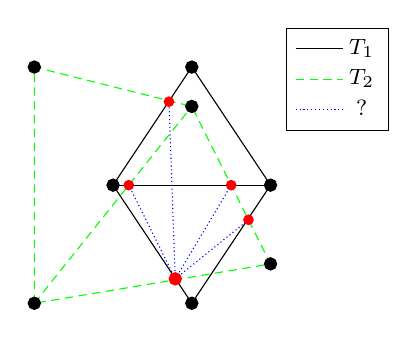
\begin{tikzpicture}
    \tikzstyle{point}=[circle,thick,draw=black,fill=black,inner sep=0pt,minimum width=4pt,minimum height=4pt]
    \tikzstyle{smallpoint}=[circle,thick,draw=red,fill=red,inner sep=0pt,minimum width=3pt,minimum height=3pt]
    \begin{pgfonlayer}{foreground}
        \node (a)[point] at (0,0) {};
        \node (b)[point] at (2,0) {};
        \node (c)[point] at (3,0.5) {};
        \node (d)[point] at (0,3) {};
        \node (e)[point] at (2,3) {};
        \node (f)[point] at (3,1.5) {};
        \node (g)[point] at (2,2.5) {};
        \node (h)[point] at (1,1.5) {};
    \end{pgfonlayer}

    \draw (h.center) -- (e.center) -- (f.center) -- (b.center) -- cycle;
    \draw (h.center) -- (f.center);

    \draw[green, densely dashed] (a.center) -- (d.center) -- (g.center) -- (c.center) -- cycle;
    \draw[green, densely dashed] (a.center) -- (g.center);

    \begin{pgfonlayer}{foreground}
        \node (x)[point, red,fill=red] at (1.79,0.31) {};
        \node (x1)[smallpoint] at (1.2,1.5) {};
        \node (x2)[smallpoint] at (1.71,2.56) {};
        \node (x3)[smallpoint] at (2.5,1.5) {};
        \node (x4)[smallpoint] at (2.72,1.06) {};
    \end{pgfonlayer}
    \draw[blue, densely dotted] (x.center) -- (x1.center);
    \draw[blue, densely dotted] (x.center) -- (x2.center);
    \draw[blue, densely dotted] (x.center) -- (x3.center);
    \draw[blue, densely dotted] (x.center) -- (x4.center);


    \begin{customlegend}[
    legend entries={
        $T_1$,
        $T_2$,
        $?$
    },
    legend style={at={(4.5,3.5)},font=\footnotesize}] % <= to define position and font legend
    % the following are the "images" and numbers in the legend
        \addlegendimage{black}
        \addlegendimage{green,densely dashed}
        \addlegendimage{blue, densely dotted}
    \end{customlegend}
\end{tikzpicture}
